The HLT shares the same code used for offline data processing, thus the processing pipeline is more or less the same. The fundamental difference is that the output is used to perform event classification instead of data analysis. 
\begin{figure}[ht]
  \centering
  \caption{HLT processing pipeline}
  \label{img:hlt}
  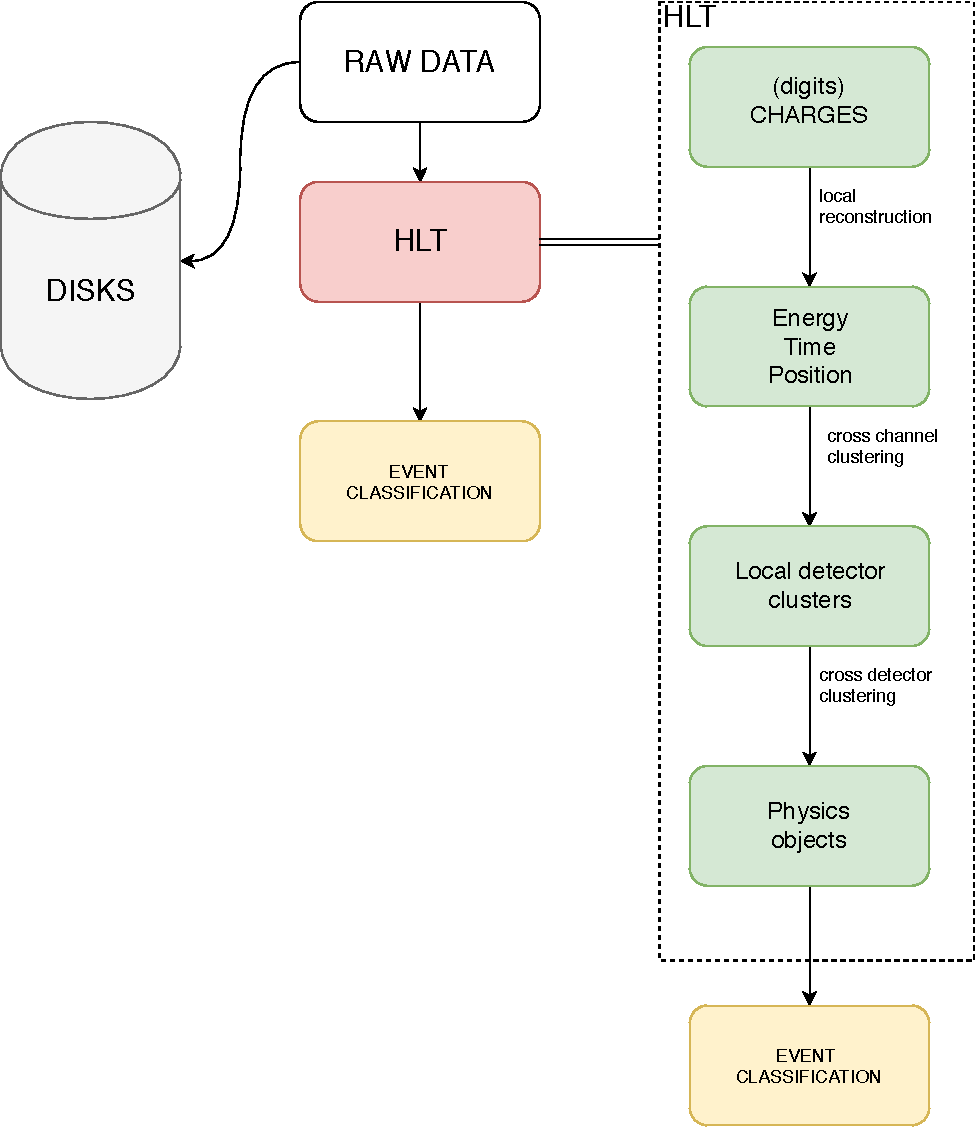
\includegraphics[width=.75\textwidth]{img/hlt}
\end{figure}
The table \ref{table:timeshare} shows how much time is spent in every single step of the reconstruction process. Most of it is spent into tracking but after it, the second more time consuming step is HCAL+ECAL local reconstruction that takes $113 ms$ corresponding to $24\%$ of the total time.
\begin{figure}[ht]
  % \centering
  \caption{Data processing time share}
  \label{img:hlt}
  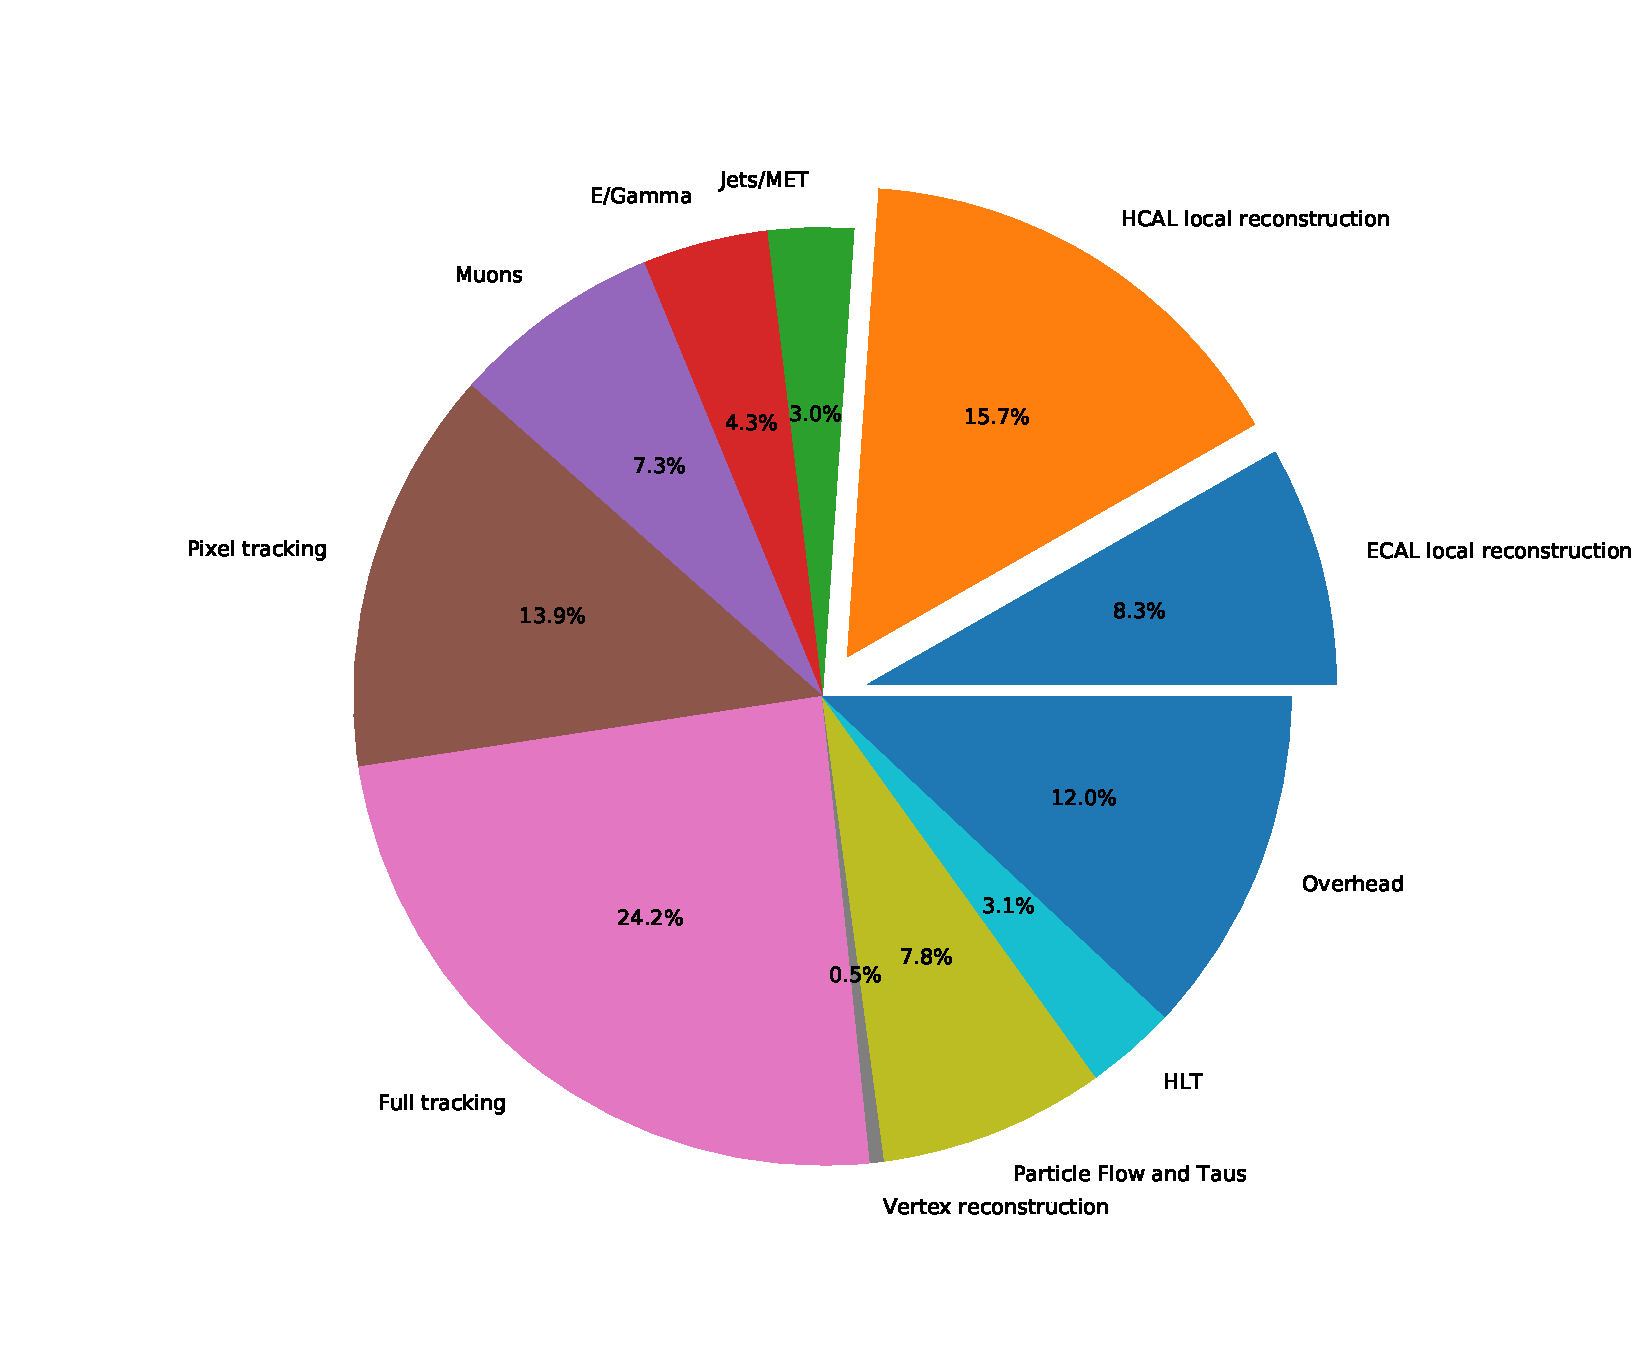
\includegraphics[width=\textwidth]{img/timeshare}
\end{figure}
Given the time needed to perform this reconstruction even achieving a speedup of two would reduce the total processing time of more than $10\%$. This is my focus in this project try to reduce it as much as possible.
\begin{table}[ht]
  \caption{Time spent into the various HLT reconstruction steps}
  \label{table:timeshare}
  \begin{tabular}{lll}
    \hline
    Step                      & Real-Time      & Percentage \\ \hline
    ECAL local reconstruction & 38.9 ms        & 8.25\%     \\
    HCAL local reconstruction & 73.9 ms        & 15.67\%    \\
    Jets/MET                  & 14 ms          & 2.97\%     \\
    E/Gamma                   & 20.4 ms        & 4.33\%     \\
    Muons                     & 34.2 ms        & 7.25\%     \\
    Pixel tracking            & 65.7 ms        & 13.93\%    \\
    Full tracking             & 114.2 ms       & 24.22\%    \\
    Vertex reconstruction     & 2.3 ms         & 0.49\%     \\
    Particle Flow and Taus    & 36.8 ms        & 7.8\%      \\
    HLT                       & 14.7 ms        & 3.12\%     \\
    Overhead                  & 56.4 ms        & 11.96\%    \\
    Total                     & 471.5 ms       & 100\%      \\ \hline
  \end{tabular}
\end{table}
\section{Problem statement}
As the name says the goal of this step is: \\
\begin{claim}
  For each channel \{given $n$ charge readouts $\rightarrow$ reconstruct the energy\}. \\
  \quad Where in this case $n$ is fixed to 10. 
\end{claim}\\
Translated into mathematical terms this means:
\begin{equation}\label{eq:01}
  \begin{split}
    & \min(\norm{Px - b}) \\
    \text{where:}&  \\
    & x = \text{energy vector} \\
    & P:CHARGE \rightarrow ENERGY =\text{feature matrix} \\
    & b = \text{charge vector}
  \end{split}
\end{equation}
As shown in \cite{amplituamplitude_reconde_recon} the statement above is incomplete. A perfect mapping from charges to energy does not exist because signal from the shower does not dissipate within one time slice ($25ns$). 
